
% Default to the notebook output style

    


% Inherit from the specified cell style.




    
\documentclass[11pt]{article}

    
    

    \usepackage[T1]{fontenc}
    % Nicer default font (+ math font) than Computer Modern for most use cases
    \usepackage{mathpazo}

    % Basic figure setup, for now with no caption control since it's done
    % automatically by Pandoc (which extracts ![](path) syntax from Markdown).
    \usepackage{graphicx}
    % We will generate all images so they have a width \maxwidth. This means
    % that they will get their normal width if they fit onto the page, but
    % are scaled down if they would overflow the margins.
    \makeatletter
    \def\maxwidth{\ifdim\Gin@nat@width>\linewidth\linewidth
    \else\Gin@nat@width\fi}
    \makeatother
    \let\Oldincludegraphics\includegraphics
    % Set max figure width to be 80% of text width, for now hardcoded.
    \renewcommand{\includegraphics}[1]{\Oldincludegraphics[width=.8\maxwidth]{#1}}
    % Ensure that by default, figures have no caption (until we provide a
    % proper Figure object with a Caption API and a way to capture that
    % in the conversion process - todo).
    \usepackage{caption}
    \DeclareCaptionLabelFormat{nolabel}{}
    \captionsetup{labelformat=nolabel}

    \usepackage{adjustbox} % Used to constrain images to a maximum size 
    \usepackage{xcolor} % Allow colors to be defined
    \usepackage{enumerate} % Needed for markdown enumerations to work
    \usepackage{geometry} % Used to adjust the document margins
    \usepackage{amsmath} % Equations
    \usepackage{amssymb} % Equations
    \usepackage{textcomp} % defines textquotesingle
    % Hack from http://tex.stackexchange.com/a/47451/13684:
    \AtBeginDocument{%
        \def\PYZsq{\textquotesingle}% Upright quotes in Pygmentized code
    }
    \usepackage{upquote} % Upright quotes for verbatim code
    \usepackage{eurosym} % defines \euro
    \usepackage[mathletters]{ucs} % Extended unicode (utf-8) support
    \usepackage[utf8x]{inputenc} % Allow utf-8 characters in the tex document
    \usepackage{fancyvrb} % verbatim replacement that allows latex
    \usepackage{grffile} % extends the file name processing of package graphics 
                         % to support a larger range 
    % The hyperref package gives us a pdf with properly built
    % internal navigation ('pdf bookmarks' for the table of contents,
    % internal cross-reference links, web links for URLs, etc.)
    \usepackage{hyperref}
    \usepackage{longtable} % longtable support required by pandoc >1.10
    \usepackage{booktabs}  % table support for pandoc > 1.12.2
    \usepackage[inline]{enumitem} % IRkernel/repr support (it uses the enumerate* environment)
    \usepackage[normalem]{ulem} % ulem is needed to support strikethroughs (\sout)
                                % normalem makes italics be italics, not underlines
    
\usepackage[round]{natbib}
\usepackage[ruled,vlined]{algorithm2e}
\usepackage{pgf}
\usepackage{tikz}
\usetikzlibrary{positioning}


    
    
    % Colors for the hyperref package
    \definecolor{urlcolor}{rgb}{0,.145,.698}
    \definecolor{linkcolor}{rgb}{.71,0.21,0.01}
    \definecolor{citecolor}{rgb}{.12,.54,.11}

    % ANSI colors
    \definecolor{ansi-black}{HTML}{3E424D}
    \definecolor{ansi-black-intense}{HTML}{282C36}
    \definecolor{ansi-red}{HTML}{E75C58}
    \definecolor{ansi-red-intense}{HTML}{B22B31}
    \definecolor{ansi-green}{HTML}{00A250}
    \definecolor{ansi-green-intense}{HTML}{007427}
    \definecolor{ansi-yellow}{HTML}{DDB62B}
    \definecolor{ansi-yellow-intense}{HTML}{B27D12}
    \definecolor{ansi-blue}{HTML}{208FFB}
    \definecolor{ansi-blue-intense}{HTML}{0065CA}
    \definecolor{ansi-magenta}{HTML}{D160C4}
    \definecolor{ansi-magenta-intense}{HTML}{A03196}
    \definecolor{ansi-cyan}{HTML}{60C6C8}
    \definecolor{ansi-cyan-intense}{HTML}{258F8F}
    \definecolor{ansi-white}{HTML}{C5C1B4}
    \definecolor{ansi-white-intense}{HTML}{A1A6B2}

    % commands and environments needed by pandoc snippets
    % extracted from the output of `pandoc -s`
    \providecommand{\tightlist}{%
      \setlength{\itemsep}{0pt}\setlength{\parskip}{0pt}}
    \DefineVerbatimEnvironment{Highlighting}{Verbatim}{commandchars=\\\{\}}
    % Add ',fontsize=\small' for more characters per line
    \newenvironment{Shaded}{}{}
    \newcommand{\KeywordTok}[1]{\textcolor[rgb]{0.00,0.44,0.13}{\textbf{{#1}}}}
    \newcommand{\DataTypeTok}[1]{\textcolor[rgb]{0.56,0.13,0.00}{{#1}}}
    \newcommand{\DecValTok}[1]{\textcolor[rgb]{0.25,0.63,0.44}{{#1}}}
    \newcommand{\BaseNTok}[1]{\textcolor[rgb]{0.25,0.63,0.44}{{#1}}}
    \newcommand{\FloatTok}[1]{\textcolor[rgb]{0.25,0.63,0.44}{{#1}}}
    \newcommand{\CharTok}[1]{\textcolor[rgb]{0.25,0.44,0.63}{{#1}}}
    \newcommand{\StringTok}[1]{\textcolor[rgb]{0.25,0.44,0.63}{{#1}}}
    \newcommand{\CommentTok}[1]{\textcolor[rgb]{0.38,0.63,0.69}{\textit{{#1}}}}
    \newcommand{\OtherTok}[1]{\textcolor[rgb]{0.00,0.44,0.13}{{#1}}}
    \newcommand{\AlertTok}[1]{\textcolor[rgb]{1.00,0.00,0.00}{\textbf{{#1}}}}
    \newcommand{\FunctionTok}[1]{\textcolor[rgb]{0.02,0.16,0.49}{{#1}}}
    \newcommand{\RegionMarkerTok}[1]{{#1}}
    \newcommand{\ErrorTok}[1]{\textcolor[rgb]{1.00,0.00,0.00}{\textbf{{#1}}}}
    \newcommand{\NormalTok}[1]{{#1}}
    
    % Additional commands for more recent versions of Pandoc
    \newcommand{\ConstantTok}[1]{\textcolor[rgb]{0.53,0.00,0.00}{{#1}}}
    \newcommand{\SpecialCharTok}[1]{\textcolor[rgb]{0.25,0.44,0.63}{{#1}}}
    \newcommand{\VerbatimStringTok}[1]{\textcolor[rgb]{0.25,0.44,0.63}{{#1}}}
    \newcommand{\SpecialStringTok}[1]{\textcolor[rgb]{0.73,0.40,0.53}{{#1}}}
    \newcommand{\ImportTok}[1]{{#1}}
    \newcommand{\DocumentationTok}[1]{\textcolor[rgb]{0.73,0.13,0.13}{\textit{{#1}}}}
    \newcommand{\AnnotationTok}[1]{\textcolor[rgb]{0.38,0.63,0.69}{\textbf{\textit{{#1}}}}}
    \newcommand{\CommentVarTok}[1]{\textcolor[rgb]{0.38,0.63,0.69}{\textbf{\textit{{#1}}}}}
    \newcommand{\VariableTok}[1]{\textcolor[rgb]{0.10,0.09,0.49}{{#1}}}
    \newcommand{\ControlFlowTok}[1]{\textcolor[rgb]{0.00,0.44,0.13}{\textbf{{#1}}}}
    \newcommand{\OperatorTok}[1]{\textcolor[rgb]{0.40,0.40,0.40}{{#1}}}
    \newcommand{\BuiltInTok}[1]{{#1}}
    \newcommand{\ExtensionTok}[1]{{#1}}
    \newcommand{\PreprocessorTok}[1]{\textcolor[rgb]{0.74,0.48,0.00}{{#1}}}
    \newcommand{\AttributeTok}[1]{\textcolor[rgb]{0.49,0.56,0.16}{{#1}}}
    \newcommand{\InformationTok}[1]{\textcolor[rgb]{0.38,0.63,0.69}{\textbf{\textit{{#1}}}}}
    \newcommand{\WarningTok}[1]{\textcolor[rgb]{0.38,0.63,0.69}{\textbf{\textit{{#1}}}}}
    
    
    % Define a nice break command that doesn't care if a line doesn't already
    % exist.
    \def\br{\hspace*{\fill} \\* }
    % Math Jax compatability definitions
    \def\gt{>}
    \def\lt{<}
    % Document parameters
    
\title{Inverse Probability of Treatment Weighting Under Violations of Positivity: Draft 2}

    
    
\author{Tomas D. Morley}

    

    % Pygments definitions
    
\makeatletter
\def\PY@reset{\let\PY@it=\relax \let\PY@bf=\relax%
    \let\PY@ul=\relax \let\PY@tc=\relax%
    \let\PY@bc=\relax \let\PY@ff=\relax}
\def\PY@tok#1{\csname PY@tok@#1\endcsname}
\def\PY@toks#1+{\ifx\relax#1\empty\else%
    \PY@tok{#1}\expandafter\PY@toks\fi}
\def\PY@do#1{\PY@bc{\PY@tc{\PY@ul{%
    \PY@it{\PY@bf{\PY@ff{#1}}}}}}}
\def\PY#1#2{\PY@reset\PY@toks#1+\relax+\PY@do{#2}}

\expandafter\def\csname PY@tok@w\endcsname{\def\PY@tc##1{\textcolor[rgb]{0.73,0.73,0.73}{##1}}}
\expandafter\def\csname PY@tok@c\endcsname{\let\PY@it=\textit\def\PY@tc##1{\textcolor[rgb]{0.25,0.50,0.50}{##1}}}
\expandafter\def\csname PY@tok@cp\endcsname{\def\PY@tc##1{\textcolor[rgb]{0.74,0.48,0.00}{##1}}}
\expandafter\def\csname PY@tok@k\endcsname{\let\PY@bf=\textbf\def\PY@tc##1{\textcolor[rgb]{0.00,0.50,0.00}{##1}}}
\expandafter\def\csname PY@tok@kp\endcsname{\def\PY@tc##1{\textcolor[rgb]{0.00,0.50,0.00}{##1}}}
\expandafter\def\csname PY@tok@kt\endcsname{\def\PY@tc##1{\textcolor[rgb]{0.69,0.00,0.25}{##1}}}
\expandafter\def\csname PY@tok@o\endcsname{\def\PY@tc##1{\textcolor[rgb]{0.40,0.40,0.40}{##1}}}
\expandafter\def\csname PY@tok@ow\endcsname{\let\PY@bf=\textbf\def\PY@tc##1{\textcolor[rgb]{0.67,0.13,1.00}{##1}}}
\expandafter\def\csname PY@tok@nb\endcsname{\def\PY@tc##1{\textcolor[rgb]{0.00,0.50,0.00}{##1}}}
\expandafter\def\csname PY@tok@nf\endcsname{\def\PY@tc##1{\textcolor[rgb]{0.00,0.00,1.00}{##1}}}
\expandafter\def\csname PY@tok@nc\endcsname{\let\PY@bf=\textbf\def\PY@tc##1{\textcolor[rgb]{0.00,0.00,1.00}{##1}}}
\expandafter\def\csname PY@tok@nn\endcsname{\let\PY@bf=\textbf\def\PY@tc##1{\textcolor[rgb]{0.00,0.00,1.00}{##1}}}
\expandafter\def\csname PY@tok@ne\endcsname{\let\PY@bf=\textbf\def\PY@tc##1{\textcolor[rgb]{0.82,0.25,0.23}{##1}}}
\expandafter\def\csname PY@tok@nv\endcsname{\def\PY@tc##1{\textcolor[rgb]{0.10,0.09,0.49}{##1}}}
\expandafter\def\csname PY@tok@no\endcsname{\def\PY@tc##1{\textcolor[rgb]{0.53,0.00,0.00}{##1}}}
\expandafter\def\csname PY@tok@nl\endcsname{\def\PY@tc##1{\textcolor[rgb]{0.63,0.63,0.00}{##1}}}
\expandafter\def\csname PY@tok@ni\endcsname{\let\PY@bf=\textbf\def\PY@tc##1{\textcolor[rgb]{0.60,0.60,0.60}{##1}}}
\expandafter\def\csname PY@tok@na\endcsname{\def\PY@tc##1{\textcolor[rgb]{0.49,0.56,0.16}{##1}}}
\expandafter\def\csname PY@tok@nt\endcsname{\let\PY@bf=\textbf\def\PY@tc##1{\textcolor[rgb]{0.00,0.50,0.00}{##1}}}
\expandafter\def\csname PY@tok@nd\endcsname{\def\PY@tc##1{\textcolor[rgb]{0.67,0.13,1.00}{##1}}}
\expandafter\def\csname PY@tok@s\endcsname{\def\PY@tc##1{\textcolor[rgb]{0.73,0.13,0.13}{##1}}}
\expandafter\def\csname PY@tok@sd\endcsname{\let\PY@it=\textit\def\PY@tc##1{\textcolor[rgb]{0.73,0.13,0.13}{##1}}}
\expandafter\def\csname PY@tok@si\endcsname{\let\PY@bf=\textbf\def\PY@tc##1{\textcolor[rgb]{0.73,0.40,0.53}{##1}}}
\expandafter\def\csname PY@tok@se\endcsname{\let\PY@bf=\textbf\def\PY@tc##1{\textcolor[rgb]{0.73,0.40,0.13}{##1}}}
\expandafter\def\csname PY@tok@sr\endcsname{\def\PY@tc##1{\textcolor[rgb]{0.73,0.40,0.53}{##1}}}
\expandafter\def\csname PY@tok@ss\endcsname{\def\PY@tc##1{\textcolor[rgb]{0.10,0.09,0.49}{##1}}}
\expandafter\def\csname PY@tok@sx\endcsname{\def\PY@tc##1{\textcolor[rgb]{0.00,0.50,0.00}{##1}}}
\expandafter\def\csname PY@tok@m\endcsname{\def\PY@tc##1{\textcolor[rgb]{0.40,0.40,0.40}{##1}}}
\expandafter\def\csname PY@tok@gh\endcsname{\let\PY@bf=\textbf\def\PY@tc##1{\textcolor[rgb]{0.00,0.00,0.50}{##1}}}
\expandafter\def\csname PY@tok@gu\endcsname{\let\PY@bf=\textbf\def\PY@tc##1{\textcolor[rgb]{0.50,0.00,0.50}{##1}}}
\expandafter\def\csname PY@tok@gd\endcsname{\def\PY@tc##1{\textcolor[rgb]{0.63,0.00,0.00}{##1}}}
\expandafter\def\csname PY@tok@gi\endcsname{\def\PY@tc##1{\textcolor[rgb]{0.00,0.63,0.00}{##1}}}
\expandafter\def\csname PY@tok@gr\endcsname{\def\PY@tc##1{\textcolor[rgb]{1.00,0.00,0.00}{##1}}}
\expandafter\def\csname PY@tok@ge\endcsname{\let\PY@it=\textit}
\expandafter\def\csname PY@tok@gs\endcsname{\let\PY@bf=\textbf}
\expandafter\def\csname PY@tok@gp\endcsname{\let\PY@bf=\textbf\def\PY@tc##1{\textcolor[rgb]{0.00,0.00,0.50}{##1}}}
\expandafter\def\csname PY@tok@go\endcsname{\def\PY@tc##1{\textcolor[rgb]{0.53,0.53,0.53}{##1}}}
\expandafter\def\csname PY@tok@gt\endcsname{\def\PY@tc##1{\textcolor[rgb]{0.00,0.27,0.87}{##1}}}
\expandafter\def\csname PY@tok@err\endcsname{\def\PY@bc##1{\setlength{\fboxsep}{0pt}\fcolorbox[rgb]{1.00,0.00,0.00}{1,1,1}{\strut ##1}}}
\expandafter\def\csname PY@tok@kc\endcsname{\let\PY@bf=\textbf\def\PY@tc##1{\textcolor[rgb]{0.00,0.50,0.00}{##1}}}
\expandafter\def\csname PY@tok@kd\endcsname{\let\PY@bf=\textbf\def\PY@tc##1{\textcolor[rgb]{0.00,0.50,0.00}{##1}}}
\expandafter\def\csname PY@tok@kn\endcsname{\let\PY@bf=\textbf\def\PY@tc##1{\textcolor[rgb]{0.00,0.50,0.00}{##1}}}
\expandafter\def\csname PY@tok@kr\endcsname{\let\PY@bf=\textbf\def\PY@tc##1{\textcolor[rgb]{0.00,0.50,0.00}{##1}}}
\expandafter\def\csname PY@tok@bp\endcsname{\def\PY@tc##1{\textcolor[rgb]{0.00,0.50,0.00}{##1}}}
\expandafter\def\csname PY@tok@vc\endcsname{\def\PY@tc##1{\textcolor[rgb]{0.10,0.09,0.49}{##1}}}
\expandafter\def\csname PY@tok@vg\endcsname{\def\PY@tc##1{\textcolor[rgb]{0.10,0.09,0.49}{##1}}}
\expandafter\def\csname PY@tok@vi\endcsname{\def\PY@tc##1{\textcolor[rgb]{0.10,0.09,0.49}{##1}}}
\expandafter\def\csname PY@tok@sb\endcsname{\def\PY@tc##1{\textcolor[rgb]{0.73,0.13,0.13}{##1}}}
\expandafter\def\csname PY@tok@sc\endcsname{\def\PY@tc##1{\textcolor[rgb]{0.73,0.13,0.13}{##1}}}
\expandafter\def\csname PY@tok@s2\endcsname{\def\PY@tc##1{\textcolor[rgb]{0.73,0.13,0.13}{##1}}}
\expandafter\def\csname PY@tok@sh\endcsname{\def\PY@tc##1{\textcolor[rgb]{0.73,0.13,0.13}{##1}}}
\expandafter\def\csname PY@tok@s1\endcsname{\def\PY@tc##1{\textcolor[rgb]{0.73,0.13,0.13}{##1}}}
\expandafter\def\csname PY@tok@mb\endcsname{\def\PY@tc##1{\textcolor[rgb]{0.40,0.40,0.40}{##1}}}
\expandafter\def\csname PY@tok@mf\endcsname{\def\PY@tc##1{\textcolor[rgb]{0.40,0.40,0.40}{##1}}}
\expandafter\def\csname PY@tok@mh\endcsname{\def\PY@tc##1{\textcolor[rgb]{0.40,0.40,0.40}{##1}}}
\expandafter\def\csname PY@tok@mi\endcsname{\def\PY@tc##1{\textcolor[rgb]{0.40,0.40,0.40}{##1}}}
\expandafter\def\csname PY@tok@il\endcsname{\def\PY@tc##1{\textcolor[rgb]{0.40,0.40,0.40}{##1}}}
\expandafter\def\csname PY@tok@mo\endcsname{\def\PY@tc##1{\textcolor[rgb]{0.40,0.40,0.40}{##1}}}
\expandafter\def\csname PY@tok@ch\endcsname{\let\PY@it=\textit\def\PY@tc##1{\textcolor[rgb]{0.25,0.50,0.50}{##1}}}
\expandafter\def\csname PY@tok@cm\endcsname{\let\PY@it=\textit\def\PY@tc##1{\textcolor[rgb]{0.25,0.50,0.50}{##1}}}
\expandafter\def\csname PY@tok@cpf\endcsname{\let\PY@it=\textit\def\PY@tc##1{\textcolor[rgb]{0.25,0.50,0.50}{##1}}}
\expandafter\def\csname PY@tok@c1\endcsname{\let\PY@it=\textit\def\PY@tc##1{\textcolor[rgb]{0.25,0.50,0.50}{##1}}}
\expandafter\def\csname PY@tok@cs\endcsname{\let\PY@it=\textit\def\PY@tc##1{\textcolor[rgb]{0.25,0.50,0.50}{##1}}}

\def\PYZbs{\char`\\}
\def\PYZus{\char`\_}
\def\PYZob{\char`\{}
\def\PYZcb{\char`\}}
\def\PYZca{\char`\^}
\def\PYZam{\char`\&}
\def\PYZlt{\char`\<}
\def\PYZgt{\char`\>}
\def\PYZsh{\char`\#}
\def\PYZpc{\char`\%}
\def\PYZdl{\char`\$}
\def\PYZhy{\char`\-}
\def\PYZsq{\char`\'}
\def\PYZdq{\char`\"}
\def\PYZti{\char`\~}
% for compatibility with earlier versions
\def\PYZat{@}
\def\PYZlb{[}
\def\PYZrb{]}
\makeatother


    % Exact colors from NB
    \definecolor{incolor}{rgb}{0.0, 0.0, 0.5}
    \definecolor{outcolor}{rgb}{0.545, 0.0, 0.0}



    
    % Prevent overflowing lines due to hard-to-break entities
    \sloppy 
    % Setup hyperref package
    \hypersetup{
      breaklinks=true,  % so long urls are correctly broken across lines
      colorlinks=true,
      urlcolor=urlcolor,
      linkcolor=linkcolor,
      citecolor=citecolor,
      }
    % Slightly bigger margins than the latex defaults
    
    \geometry{verbose,tmargin=1in,bmargin=1in,lmargin=1in,rmargin=1in}
    
    

    \begin{document}
    
    
    \maketitle
    
    

    
    \newpage

\section{Abstract}\label{abstract}

In this thesis we study the performance of the inverse probability of
treatment weighted (IPTW) for marginal structural models under
violations of the positivity assumption. To our knowledge the
performance of MSMs under violations of this assumption have not been
systematically studied in the litrature. We employ the simulation
algorithm of \citet{Havercroft2012} to generate data in a typical
longitudinal setting. By exploiting the design of this algorithm it is
possible to introduce positivity violations that are propagated through
patient histories and study the effect of these violations on the
ability of a marginal structural model to recover the true parameters.
Our results suggest that even small violations of the positivity
assumption can have a large impact on the performance of the estimation.

    \newpage

\section{Acknowledgements}\label{acknowledgements}

    \newpage

\tableofcontents{}

    \newpage

\section{Section 1: Introduction}\label{section-1-introduction}

Marginal structural models (MSMs) are a popular class of models for
performing causal inference in the presence of time dependent
confounders. These models have an important application in areas of
research such as epidemiology, social sciences and economics where
randomised trials are prohibited by ethical or financial considerations.
Under these circumstances confounding can obscure the causal effect of
treatment on outcome. An example of this, common in epidemiological
studies, occurs when prognostic variables inform treatment decisions
while at same time being predictors of the outcome of interest. In a
longitudinal setting this is further complicated when the confounder
itself is determined by earlier treatment. One consequence is that
regression adjustment methods do not control for confounding in the
longitudinal case and other techniques are required. A second
consequence is that simulating data from a specific marginal structural
models is more challenging when the data is to exhibit time dependent
confounding.

The Inverse probability of treatment weighting (IPTW) estimator is a
technique that has been applied to censoring, missing data and survey
design problems. The central idea is that by weighting the observed
data, a pseudo population is constructed from which inference on the
target population can be achieved. For example, when there is missing
data weights can be used to create a pseudo-population in which there is
no missingness. In the context of MSMs, the IPT weights relate to a
pseudo-population in which there is no longer any confounding between
the confounder and treatment and causal inferences can be made.

Underlying IPTW are three assumptions: 1) exchangeability 2) positivity
3) and correct model specification. The focus of this thesis will be on
violations of the positivity assumption. Positivity means that within
every strata spanned by the confounders, there must be a positive
probability of patients being exposed or unexposed to treatment. For
example, in a medical context, if treatment protocols demand that
treatment is initiated whenever a prognostic variable falls below a
pre-defined threshold, there will only be exposed and no unexposed
patients in this strata of the confounding prognostic variable. make
decisions based on protocols positivity can be. In the absence of
structural positivuty violations, there is always the threat that random
zeroes arise in some strata of the confounder especially when the sample
size is small or the number of confounding variables is large. In each
case the sparsity of data within the strata of the confounder results in
a high chance that positivity is violated. Positivity violations
increase the bias and variance of estimates of the causal effect but the
extent of the damage is not well known. The central aim of this thesis
will be to investigate positivity violations when fitting MSMs to
longitudinal data. To our knowledge positivity violations have not been
systematically studied in the literature from a simulation point of
view. We quantify the bias and variance introduced due to positivity
violations and hope to provide practical advice to researchers tempted
to fit MSMs to overcome confounding without realising the potential
consequences of positivity violations in their data.

Throughout this thesis we focus on clinical applications as examples. In
the literature on marginal structural models the causal effect of
Zidovudine on the survival of HIV positive men is often cited as an
example. In this example a patients white blood cell (CD4) count is a
prognostic variable that influences a doctor's decision to initiate
treatment while at the same time being a predictor of survival. As a
result CD4 count is a confounder. In the longitudinal setting previous
treatments influence CD4 count. As such studies often depend on
protocols which means that poistivity in some levels of the confounder
make this a suitable example for our purposes.

The structure of this thesis is as follows. In section 2 of part 1, the
model considered in this thesis and its important aspects are explained.
In part 2 simulating from this statistical model is discussed in detail.
In part 3 the model under dynamic strategies is considered and
comparisons are drawn with the static case. In part 4 we entertain
violations of positivity in the data, this section represents the
novelty in this thesis. Part 5 conducts a simulation study. Part 6
includes a discussion, conclusions and suggestions for future work.

    \subsubsection{Directed Acyclic Graphs}\label{directed-acyclic-graphs}

In this thesis we consider simulating from marginal structural models
(MSMs), a class of models that can be used to estimate causal effects
from observational data under time dependent confounding. Specifically,
we consider the problem, common in medical research, of investigating
the relationship between a binary treatment variable \(A\) and an
outcome of interest \(Y\) in the presence of a covariate \(L\). One way
of expressing the relationship between these three variables is through
a graph such as the one shown in the left hand size of figure 1.

A graph consists of a finite set of vertices \(\nu\) and a set of edges
\(\epsilon\). The vertices of a graph correspond to a collection of
random variables which follow a joint probability distribution
\(P(\nu)\). Edges in \(\epsilon\) consist of pairs of distinct vertices
and denote a certain relationship that holds between the variables
\citet{Pearl2009}. The direction of the relationship is denoted by an
arrow and in this thesis we consider only acyclic graphs which means
that the relationship between two variables only proceeds in one
direction, there are no feedback loops or mutual causation. The
resulting directed acyclic graph (DAG) \(G = (\nu, \epsilon)\) shown in
figure 1 can be represeted as a set of connections \({(A, Y), (L, Y)}\)
where direction is from the first element of each pair to the second
element.

    \subsection{Time Dependent
Confounding}\label{time-dependent-confounding}

The right hand side of figure 1 represents the confounding case where
the DAG \(G\) has been ammended to include a relationship from \(L\) to
\(A\) \(G = {(A, Y), (L, Y), (L, A)}\). This confounding relationship
precludes causal inference because we cannot discern the relationship
between treatment \(A\) on outcome \(Y\) when \(L\) is a common cause of
both. If \(L\) is the only confounder and there are no unmeasured
confounders, then it is possible to correctly estimate the causal
relationship between \(A\) and \(Y\) by adjusting for the measured
confounders.

The time dependent case adds another complication which is a further
relationship between previous treatment \(A_{t-1}\) and \(L_t\) as shown
in figure 2.

Talk about the minimum required to deal with the time dependent case.
Data on all time independent and time dependent variables. correct model
specification. Explain why time dependent as opposed to time independent
(baseline - do not change over time) variables are more of a problem.

By blocking the pathway between A -\textgreater{} L -\textgreater{} Y at
L, we get distorted estimates of the effect of treatment on outcome.

In the one-shot case the outcome \(Y\) depends on the treatment
decision, measured covariates and unmeasured covariates. In the
longitudinal case, the outcome depends on the histories of the treatment
and covariates. One complication is that current values of the covariate
may depend on previous treatments, and previous treatments may, in turn,
depend on previous covariates. If treatment is succesful this will
inform future treatments and also affect the outcome of interest \(Y\).
While in the one-shot case in figure 1 regression adjustment using

Allow for the joint determination of outcomes and treatment status or
omitted variables related to both treatment status and outcomes (Angrist
2001).

Similarily, if treatment is succesful this will affect both the outcome
and subsequent treatments. Analogous to the one-shot case,
\(P(y\ |\ \bar A= \bar a) \ne P(y\ |\ do(\bar A = \bar a))\). Regression
adjustment will always introduce other sources of bias in the time
dependent case. As a result regression adjustment does not work. Only
the IPTW method adjust for selection bias and confounding.

A covariate \(L\) is a confounder if it predicts the event of interest
and also predicts subsequent exposure. Explain how this actually
happens, as U0 is a common ancestor of A through L and also Y, also that
there is selection bias, and L is sufficient to adjust for confounding
see Havercroft algorithm code page bottom.

The reason why U is important is because with U, we can obtain any
P(Y~\textbar{}~do(a))\$ using the inverse of U?? We can do this under
any counterfactual survival path.

Explain why there will always be selection bias, and hence there will
always be a form of confounding in a longitudinal model.

    \subsubsection{Marginal structural
models}\label{marginal-structural-models}

Marginal structural models are a class of models which can be used to
estimate causal effects in the presence of time dependent confounding.
They model the marginal distribution of counterfactual variables over
any covariates and are referred to as structural because in econometric
and social sciences literature the term structural is often used in
place of causal \citet(hernan, brumback and robins). An oft cited
observational outcome in statistics without a causal relationship is
umbrella sales and the probability of rain. A counterfactual outcome is
broader, it encompasses not only the outcome when umbrella sales are
purchased in high volumes but also when they are not. Intuitvely the
connection between counterfactuals and A counterfactual variable for
\(Y\) is the random variable consisting of a subjects outcome under a
\(A\) regardless of whether the subject actually received this treatment
or not. Juxtaposed to an observational outcome, a counterfactual outcome
... correspondingly, the probability recorded for a subject. In the
observational case, given the treatment and . Within the context of a
MSM, the focus is the causal relationship that exists between treatment
and outcome. The following from \citet{Pearl2009} defines a causal
relationship.

\paragraph{Definition 1}\label{definition-1}

(Def 3.2.1 from \citet{Pearl2009}, abridged) Given two disjoint sets of
variables, A and Y, the causal effect of \(A\) on \(Y\), denoted as
\(P(y\ |\ do(A=a))\), is a function from X to the space of probability
distributions on \(Y\). For each realization \(a\) of \(A\),
\(P(y\ |\ do(A=a))\) gives the probability that \(Y=y\) induced by
deleting from the model all equations corresponding to variables in
\(A\) and substituting \(a\) into the remaining equations.

Associative models like regression models model the conditional
distribution \(P(Y\ |\ A=a, L=l)\)

Have been used for missing data problems. see pp.442 of Hernan,
Brumback, Robins 2001 for a list of papers linked to this

structural is only in the MSM name because structural is used in
econometrics and social science. Structural here only means that it is a
causal model.

Counterfactuals, breeze through this ...

A MSM When a relationship exists between \(L\) and \(A\) as in the right
hand side of figure 1 then there is a confounding relationship and
associative models will not have a causual interpretation. The following
definition from \citet{Pearl2009} defines what is meant by a causal
effect:

An example of this definition involves deleting the link between L and A
in the diagram.

An associative model like a regression model.

When treatments are randomised this is not a problem This might arise,
for example, when the decision to instigate treatment is based on a
measured covariate \(L\). Contrast this to randomized controlled trial,
where due to the randomization process treatment will be independent of
any measured or unmeasured covariates. The randomized controlled trial
does not often arise in epidemiology, social sciences or econometrics
due to prohibitive ethical or financial concerns. As a result other
methods are sought in order to uncover the causal effects. Marginal
structural models are a class of models which make it possible to
estimate the causal effect of \(A\) on \(Y\) in the presence of
confounders.

\begin{itemize}
\tightlist
\item
  still have unmeasured confounders of course. Or model mispecification.
  Either of these mean that results no longer hold.
\end{itemize}

A model that parameterises \(P(Y\ |\ do(A=a))\) is called a marginal
structural model (MSM) as it is marginal over any covariates and
structural in the sense that it represents an interventional rather than
observational model. The distinction between an interventional and
observational model is expressed in definition 1.1 through the notation
\(do(a)\) in \(P(y\ |\ do(x))\), as opposed to the observational case
\(P(y\ |\ A=a)\).

marginal structural models are usually for counterfactuals
-\textgreater{} example -\textgreater{} straight through to the IPW not
too much on counterfactuals.

    \begin{figure}
\centering

\begin{minipage}{.2\textwidth}

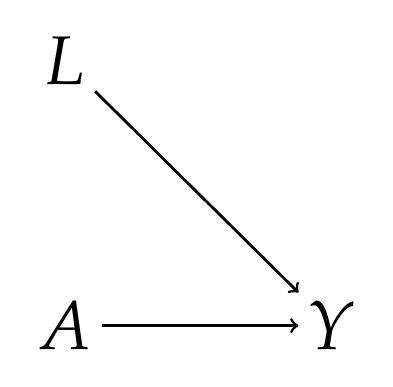
\begin{tikzpicture}

\tikzstyle{every node}=[font=\Huge]

% nodes %
\node[text centered] (a) {$A$};
\node[right = 2.5 of a, text centered] (y) {$Y$};
\node[above= 2.5 of a, text centered] (l) {$L$};

% edges %
\draw[->, line width= 1] (a) --  (y);
\draw [->, line width= 1] (l) -- (y);

\end{tikzpicture}

\end{minipage}
\hspace{3cm}% NO SPACE!
\begin{minipage}{.2\textwidth}

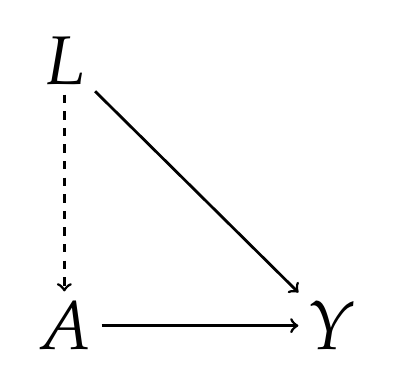
\begin{tikzpicture}

\tikzstyle{every node}=[font=\Huge]

% nodes %
\node[text centered] (a) {$A$};
\node[right = 2.5 of a, text centered] (y) {$Y$};
\node[above= 2.5 of a, text centered] (l) {$L$};

% edges %
\draw[->, line width= 1] (a) --  (y);
\draw [->, line width= 1] (l) -- (y);
\draw [->, line width= 1, dashed] (l) -- (a);

\end{tikzpicture}

\end{minipage}
\caption{Figure 1 DAG} \label{fig:fig2}
\end{figure}

    An example of this distinction is the effect of Zidovudine on the
survival of HIV-positive men. Of interest is the effect that Zidovudine
has on survival. This is what we want to estimate and it is captured in
the DAG in figure 1 as the edge connecting A and Y.

importantly, changing the relationship between L and A, won;t change the
relationship between L and Y. This means that an intervention in \(A\)
does not affect the relationship between \(L\) and \(Y\). So we remove
the link between \(L\) and \(A\) and assign to \(A\) the value of
treatment on or off. Once we place the patient on treatment, regardless
of the relationship which had existed before hand between the covariate
and treatment, a new relationship between \(A\) and \(Y\) exists in
which the covariate has no say.

This distinction can be understood more clearly when comparing
randomized controlled trials in medical resarch and observational
epidemiological research. In randomised trials the In the presence of
confounding \(P(y\ |\ A=a)\) will not represent the true causal effect
of \(A\) on \(Y\) why?. The interventional case \(P(y\ |\ do(A=a))\), on
the otherhand, \(\ne P(y\ |\ do(x))\) with the result that a model which
is conditional on A will not represent the true causal effect of A on Y.
In the former case the system is changed such that variable A takes on a
particular value or history, the result represents the system under the
intervention \(do(A=a)\) (pearl 2010). On the other hand the first
method represents the situation where the model is unchanged and \(A\)
is observed to be \(a\). This distinction will be particularly important
when considering static and dynamic stratgeies in subsequent sections.

From the point of view of simulating from a marginal structural model,
In a nutshell, we need a simulation algorithm that allows us to simulate
discrete time longitudinal data in which A affects Y, and so does L and
L affects A. The most direct way of doing this would be the red line in
the DAG. But this won't do in our case. The Havercroft and Didelez
algorithm is useful because it allows us to break the relationship
between L and A. We need to do this in such a way that we do not change
the relationship between Y and L, although we are not so interested in
this relationship because it is the least interesting of the
relationships in the diagram.

    \subsection{Simulating from a MSM}\label{simulating-from-a-msm}

Problem statement: SImulating from a given marginal structural model is
challenging because a direct relationship between L and Y would ...

The relationship between Y and L is then dependent on A. There is no
relationship between A and U because of the set-up in the DAG. The
variable L blocks this relationship.

In their paper \citet{Havercroft2012} develop an algorithm that allows
simulating data that corresponds to a particular parameterisation of an
MSM. This algorithm provides the bedrock of the simulation structure
considered in this thesis. Figure 1 represents the system under
consideration. The DAG in figure 1 represents the one-shot
non-longitudinal case. Factorising the joint distributions of the
variables in figure 1 yields

\[P(U,\ L,\ W,\ A,\ Y) = P(W)P(U)P(W)P(L\ |\ U)P(A\ |\ L,W)P(Y\ |\ U,A)\]

Where, following definition 1.1 we delete \(P(A\ |\ L,W)\), a
probability function corresponding to \(A\), and replace \(A=a\) in all
remaining functions

\[ P(U, L, W, Y\ |\ do(A=a)) =
  \begin{cases}
    P(U)P(L\ |\ U)P(Y\ |\ U,A = a) & \quad \text{if } A = a\\
    0  & \quad \text{if } A \neq a\\
  \end{cases}
\]

The goal is to simulate from a particular MSM. This means parameterising
\(P(Y\ |\ do(A=a))\). Applying the law of total probability over \(W\),
\(U\) and \(L\) yields

\[P(Y\ |\ do(A=a) = \sum_{w, u, l} P(W)P(U)P(L\ |\ U)P(Y\ |\ U, L, A=a) = \sum_{u, l} P(U)P(L\ |\ U)P(Y\ |\ U, L, A=a)\]

Making use of the fact that
\(P(L, U) = P(L\ |\  U)P(U) = P(U\ |\ L)P(L)\) and summing over either W
and U or W and L yields

\[P(Y\ |\ do(A=a) = \sum_{l}P(Y\ |\ L, A=a)P(L) = \sum_{u} P(Y\ |\ U, A=a)P(U))\]

If we can find suitable forms for either \(P(Y\ |\ L, A=a)\) and
\(P(L)\) or \(P(Y\ |\ U, A=a)\) and \(P(U)\) that correspond to the MSM
\(P(Y\ |\ do(A=a)\), then, given suitable values for \(A, L, U\) it will
be possible to simulate from the chosen MSM.

use the phrase, "in words ...." to make something more understandable.

Choosing a functional form for \[P(Y\ |\ do(A=a)\] depends on
convenience. We need a functional form that can be easily represented by
\(P(Y\ |\ L, A=a)P(L)\). non-linear functions will be hard to work into
the analysis.

U \textasciitilde{} U{[}0, 1{]} is a good choice because we can usethe
CDF of Y because U{[}0, 1{]} is always between 0 and 1

General health is patient specific but comes from a clear distribution
and has a nice medical interpretation. In contrast L would be more
difficult to include. It is better as a function of U than a value in of
itself.

    \subsection{Inverse Probability
Weighting}\label{inverse-probability-weighting}

Three assumptions behind IPTW Interval censoring is an example of IPTW
but not of marginal structural models. Cite the horowitz Thompson
estimator. Invers probability of treatment weighted estimators are a
class of estimators with applications to missing data problems,
censoring and marginal structural models.

Inverse Probability of Treatment Weighting (IPTW) is a method for
estimating MSMs in the presence of time dependent confounding. For each
observation a weight is calculated which can be thought of informally as
the inverse of the probability that a patient receives their own
treatment. This has the effect of creating a pseudo population
consisting of \(w_i\) copies of each subject \(i\) where \(w_i\) are the
IPT weights. In the pseudo population A is no longer confounded with L
and crucially \(P(Y = 1\ |\ A)\) is the same as the true population
values \citet{Robins2000}.

IN previous simulation studies unstabilized weights show substantial
increase in SEs

Weightin creates a pseudo -population in which the exposure is
independent of the \textbf{measured} confounders (Hernan, Cole, 2008)
The weight is informally proportional to the participants probability of
receiving her own exposure history

As these weights have high instability we need to stabilize them. The
unstabilized weights can be driven by only a small number of
observations. Under time dependent confounding it may still be possible
to recover the causal effect of \(A\) on \(Y\) by the method of Inverse
Probability of Treatment (IPT) weihting. How does this work?

\begin{itemize}
\tightlist
\item
  true weights are unknown but can be estimated from the data.
\item
  Robins(2000) - when there are no unmeasured confounders, we can
  control for confounding using weights
\item
  weighting adjusts for confounding and selection bias due to mesured
  time varying covariates affected by prior exposure.
\item
  \(A_t\) is no longer affected by \(L_t\), and crucially the causal
  effect of \(\bar A\) on \(Y\) remains unchanged
\end{itemize}

No unmeasured confounding time dependent confounding in the set-up we
consider, will always introduce bias. In the time dependent case, we
will therefore always have bias. And IPT weighting a means of avoiding
this.

treatment increases/imporves L and this in turn affects the probaility
of getting treatment A.

lack of adjustment for L precludes unbiased estimation. This is because
it introduces selection bias.

Problem is that the weights will have very high variability, so we need
to stabilize them otherwise they will affect the estimates. Explain all
the little details about why it becomes more variable etc. IPTW is a
method of correcting for time dependent confounding when fitting
marginal structural models.

No matter whether we use stabilized or unstabilized weights, under
positivity violations the weights will be undefined.

By including the weights we can then include regress Y on A in a model
that does not include L at all. This is important for the MSM above,
because if we choose the model conditional on L, we lose the L
altogether and just have a model conditional on A.

Conditions under which IPTW work are largely untestable (westreich 2012)

Informally a patients weight through visit k is proportional to the
inverse of the probability of having her own exposure history through
visit k (Cole and Hernan 2008)

Be more specific about what is contained in the weights. The denominator
depends on the measured confounders \(L\) the numerator does not, but
could contain baseline coefficients in the numerator to help stabilize
the weights.

weighted regression and MSM are equivalent.

L0 and baseline values - make sure that B = baseline and L0 are either
together, or have them clearly split. V is a variable predictive of A
but not of Y - hence not a confounder No rebalancing the baseline
covariates like gender or age (B), so if we want to see the effect of
groups of basline If we do not condition on baselines like age then we
break the link between age and treatment. So baselines must be in the
condition.

    \subsection{Static vs. Dynamic
Strategies}\label{static-vs.-dynamic-strategies}

So far we have considered static strategies, in this section we
desbcribe the differences between static and dynamic strategies. A
static stratgey is one where the value where the values that \(A\) will
take depend on for A is represented as:

Where a(t) = 1 if the strategy specifies that a is to take the value 1
at time \(t\). In contrast, a dynamic regime is any well-specified way
of adjusting the choice of the next decision(treatment or dose to
administer) in the light of previous information constitutes a dynamic
decision (or treatment) strategy (Didelez arxiv).

To our knowledge positivity violations in the dynamic case have not been
considered in the literature.

Hernan etal (2005) for looking at comparing dynamic regimes using
artificial censoring.

    \subsection{Positivity}\label{positivity}

Estimating the weights described in the previous section relies on four
assumptions of consistency, exchangeability, positivity and non
mispecification of the model \citet{Cole2008}. In this thesis we examine
the effect of positivity violations on our ability to recover the true
model parameters from a given MSM.

Positivity is the condition that in every strata of the covariates there
is a non-zero probability of receiving each level of treatment. In the
one shot case represented by the DAG in figure 1 this would correspond
to the formal statement \(P(A\ |\ A_0, L) > 0\) while in the
longitudinal case, incorporating the histories of the treatment and
covariates, the positivity assumption can be stated

\[P_\tau(A_\tau\ |\ \bar A_{\tau-1}, \bar L_{\tau}) > 0\]

Also need to condition on survival up to the present time.

When this is not met, the weights will be undefined, and the resulting
estimates will be biased.

from Westreich 2012: positivity requires that there are treated and
untreated individuals at every combination of the values of the
confounders at every combination of the values of the confounders in the
observed data.

Positivity can be violated if, for example, medical protocols demand
that a doctor always treat a patient if a risk factor falls below a
certain threshold. there are both exposed and unexposed individuals at
every level of the confounders (Cole, Hernan, 2008). If positivity is
violated because doctors have protocols to treat patients when L falls
below a certain level, then positivity is violated. If the structural
bias occurs within levels of a time-dependent confounder then
restriction or censoring may lead to bias whether one uses weighting or
other methods (Cole and Hernan 2008). In fact, weighted estimates are
more sensitive to random zeroes (Cole, Hernan, 2008)

When positivity is violated, the weights are undefined because .... In
this case the weights may lead to a biased estimate of the causal effect
of A on Y. Examining the extent of this bias in MSMs will be the central
purpose of this thesis.

\paragraph{Definition 2: positivity}\label{definition-2-positivity}

(Appendix 2 Cole and Hernan 2008): Positivity states that there is a
non-zero (i.e. positive) probability of receiving every level of
exposure \(X_{ij}\) for every combination of values of exposure and
covariate histories that occur in individuals histories.

In section V we will consider violations of positivity to examine the
extent of the bias introduced into the estimates when the assumption of
positivity is not met. The inverse probability weights are equal to the
stanilized weights, only if positivity holds. If positovity does not
hold, the weights are undefined and may result in biased estimates of
the causal effects.

As described above, the model only holds as long as key assumptions are
met, and one of these is positivity. Introducing violations of
positivity can be achieved by censoring observations.

\begin{itemize}
\tightlist
\item
  Point out difficulty in simulation from this model.
\item
  talk about blocking a back door from U to Y?
\item
  Pearl and Robins (1995) probabilistic evaluation of sequential plans
  from causal models with hidden variables.
\end{itemize}

    \subsection{Related work}\label{related-work}

\begin{enumerate}
\def\labelenumi{\arabic{enumi}.}
\tightlist
\item
  On MSMs - mainly hernan and Robins
\item
  On other work into positivity
\item
  On Simulating from MSMs
\end{enumerate}

Marginal Structural Models

The aim is to be able to simulate the survival function of a desired MSM
under the intervention \(do(\bar a)\)

Several studies have developed algorithms for simulating data from
marginal structural models in the presence of time dependent
confounding. An early example is \citet{bryan2004} who study estimators
of the causal effec of a time dependent treatment on survival outcomes.
They compare naive estimators with IPTW and a treatment orthogonalized
estimator which is also developed in the paper. This study shares
similarities with \citet{Havercroft2012}

\begin{itemize}
\item
  stay on treatment after treatment starts
\item
  treatment regime is determined by t* (starting point of treatment
  because it is a vector of \{0, 0, 0, 1, 1, 1\}
\item
  they motivate a logistic model for the haxard function, they use a
  discrete equivalent to the hazrd function (link to citation about
  farington study.)
\item
  the survival time U is directly linked to the survival outcome
  -\textgreater{} here it is good to provide more inuition.
\item
  need to understand why it is linked.

  Work that proposes a different method to solve the same problem. Work
  that uses the same proposed method to solve a different problem. A
  method that is similar to your method that solves a relatively similar
  problem. A discussion of a set of related problems that covers your
  problem domain.
\end{itemize}

These previous studies have lacked a systematic investigation of
positivity violations in a simulation setting. It is unknown, for
example, how large an effect a violation of positivity has and how it is
affected by the sample siz, threshold etc etc.

\begin{enumerate}
\def\labelenumi{\arabic{enumi}.}
\item
  marginal structural models literature
\item
  Simulating from marginal structural models
\item
  positivity
\item
  connect limited work on simulating from models to positivity
\item
  Explain why we choose the Havercroft simulation of the others,
  specifically why it helps us to incorporate violations of positivity
  in our analysis.
\end{enumerate}

Bryan etal 2010 have a similar focus as Havercroft 2012 in that they
develop an algorithm for simulation from a given MSM and they use this
algorithm to compare IPTW methods to naive regression methods.

Several studies have considered simulation from margial structural
models. The finite-sample properties of marginal structural proportional
hazards models has been considered by \citet{Westreich2009}.

\begin{itemize}
\tightlist
\item
  What is their focus?
\item
  how do they simulate
\item
  what do they find (in terms of MSE, SE, etc.
\item
  how does it differ from HD (2012)
\end{itemize}

Young etal (2014) also provide a simulation algorithm for simulating
longitudinal data from a known Cox MSM.

\begin{itemize}
\tightlist
\item
  What is their focus?
\end{itemize}

to compare IPW and standard regression based techniques. This is not the
subject of this thesis.

Comparing IPW and standard regression based estimates in the absence of
model misspecification. This allows for complete isolation of any type
of bias. This approach involves simulating data from a standard
parametrization of the likelihood and solving for the underlying Cox MSM

\begin{itemize}
\item
  how do they simulate
\item
  what do they find (in terms of MSE, SE, etc.
\item
  how does it differ from HD (2012)
\end{itemize}

we describe an approach to Cox MSM data generation that allows for a
comparison of the bias of IPW estimates versus that of standard
regression-based estimates in the complete absence of model
misspecification

\begin{itemize}
\tightlist
\item
  could do this section in comparison to Havercroft and didelez, explain
  how their algorithm works first and then describe the related work by
  linking differences in their algorithm to earlier or other algorithms.
\end{itemize}

ALgorithm:

\begin{enumerate}
\def\labelenumi{\arabic{enumi}.}
\item
  generate survival under no treatment from a weibull
\item
  generate survival times under the ten non-zero treatment levels.
\item
\end{enumerate}

Bryan et al (2010) Cole (2008) for more of a discussion about
positivity, with an actual observed data example. While Cole (2008) have
looked at positivity in an observational setting, to our knowledge no
study has looked at positivity violations within a simulation setting.

Cole and Hernan 2008 have examined the four assumptions underlying IPW
using a study on real data from the HAART SWISS study.

\begin{enumerate}
\def\labelenumi{\arabic{enumi}.}
\tightlist
\item
  2 paper on simulation + Bryan paper - why this simulation method is
  different from other sim papers
\item
  related work - Judea pearl, Robins, econometrics, related and broader
  literature on MSM
\item
  positivity long discussion in Hernan and cole and the warnings but no
  simulation study in that paper. They study the positivity but not the
  effect and there is nothing in the havercroft paper on this either.
\end{enumerate}

\begin{itemize}
\item
\item
  Major point is that there are a number of ways of simulating from
  marginal structural models. But, we need one where we can mess with
  the positivity. Other methods are not suitable for this.
\item
  G formula simulation
\item
  exposure, confounder feedback loop
\item
  treatment
\item
  outcome variable
\item
  causal effect of the treatment variable on the outcome.
\item
  external intervention
\item
  Explain the do notation, and what presicely is meant in the case\\
\item
  used to estimate the joint effect of time dependent treatments on
  survival
\item
  Need to stronly link the time dependent confounding to the MSM, do we
  choose this class of models because of their relationship with time
  dep confounding? Yes, marginal strictural models are used with TDC
\item
  The causal graph helps (according to Pearl pp. 40) to bridge
  statistics into causality
\item
  There is a key part to this, which is that we do not observe
  confounding, this seems to be what motivates the use of the MSM class
  of models.
\item
  Counterfactuals need to be addressed here to make it clear this is not
  the purpose of the thesis.
\item
  Robins (2000) have demonstrated that in the presense of time dependent
  confounders, standard approaches for asjusting for confounding are
  biased.
\item
  A covariate that is a risk factor for, or predictor of the event of
  interest (Y) (from Robins 2000). This defines a time dependent
  covariate
\item
  And also past exposure determines the level of the covariate.
\item
  Works under a set of assumptions (consistency, exchanchability,
  positivity and no mispecification of the model used to estimate the
  weights
\item
\end{itemize}

    \section{Chapter 2}\label{chapter-2}

\subsection{Simulating from a static
MSM}\label{simulating-from-a-static-msm}

\subsection{Data Structure}\label{data-structure}

We wish to simulate survival data in discrete time \(t = 0, \dots, T\)
for \(n\) subjects. At baseline \(t=0\) all subjects are assumed to be
at risk of failure so that \(Y_0 = 0\). For each time period
\(t = 0, \dots, T\) a subject may either be on treatment, \(A_t = 1\),
or not on treatment, \(A_t = 0\). All patients are assumed to be not on
treatment before the study begins. Once a patient commences treatment,
they remain on treatment in all subsequent periods until failure or the
end of follow-up. In each time period \(L_t\) is the value of a
covariate measured at time \(t\). In the simulated data, \(L_t\) behaves
in a similar manner to CD4 counts such that a low value of \(L_t\)
represents a more severe illness and hence a higher probability of both
tratemnt and failure in the following period. In addition to \(L_t\),
the variable \(U_t\) represents subject specific general health at time
\(t\). Although we will simulate \(U_t\), in a real world application
\(U_t\) is an unmeasured confounder which

Each time period is either a check up visit or is between two check up
visits. If \(t\) is a check-up visit and treatment has not yet
commenced, \(L_t\) is measured and a decision is made on whether to
commence treatment. Between visits, treatment remains unchanged at the
value recorded at the previous visit. Similarly, \(L_t\) which is only
measured when \(t\) is a visit, alos remains unchanged.

We represent the history of a random variable with an over bar. For
example, the vector representing the treatment history of the variable A
is represented by \(\bar A = [a_0, a_1, \dots, a_m]\) where \(m=T\) if
the subject survives until the end of follow-up, or \(m < T\) otherwise.
Prior to basline both \(A = 0\) for all subjects.

\begin{itemize}
\tightlist
\item
  explain what \(U\) is and how it relates to the simulation
  design/algorithm
\item
  Be more specific on \(Y\)
\item
  L\_t is a measured confounder
\item
  U\_t is an unmeasured confounder.
\end{itemize}

\subsection{Simulation Algorithm}\label{simulation-algorithm}

\subsubsection{Algorithm}\label{algorithm}

Next, we describe the algorithm used to simulate data from our chosen
marginal structural model under time dependent confounding. In the
following section we discuss in detail how the algorithm works and the
salient features for this thesis. The algorithm is taken from
\citet{Havercroft2012} who generate data on \(n\) patients, for \(k\)
time periods. The outer loop in the following algorithm
\(i \in {1, \dots, n}\) , refers to the patients while the inner loop
\(t \in {1, \dots, T}\) refers to the subsject specific time periods
from baseline to failure or the end of the study. There will be at least
one, and at most \(T\) records for each patient.

\begin{algorithm}[H]
\SetAlgoLined
\KwResult{Marginal Structural Model Under Time Dependent Confounding}
 \For{i in 1, \dots , n}{
  $U_{0, i} \sim U[0, 1]$\\
  $\epsilon_{0, i} \sim N(\mu, \sigma^2)$\\
  $L_{0, i} \gets F^{-1}_{\Gamma(k,\theta)}(U_{i, 0}) + \epsilon_{0, i}$\\
  $A_{-1, i} \gets 0$\\
  $A_{0, i} \gets Bern(expit(\theta_0 + \theta_2 (L_{0, i} - 500)))$\\
  \If{$A_{0, i}= 1$}{
   $T^* \gets 0$;
  }
  $\lambda_{0, i} \gets expit(\gamma_0 + \gamma_2 A_{0, i})$\\
  \eIf{$\lambda_{0, i} \ge U_{0, i}$}{
   $Y_{1, i} \gets 0$\\
   }{
   $Y_{1, i} \gets 1$\\
  }
  \For{$k in 1, \dots , T$}{
   \If{$Y_{t, i} = 0$}{
    $\Delta_{t, i} \sim N(\mu_2, \sigma^2_2)$\\
    $U_{t, i} \gets min(1, max(0, U_{t-1, i} + \Delta_{t, i}))$\\
    \eIf{$t \neq 0\ (mod\ k)$}{
     $L_{t, i} \gets L_{t-1, i}$\\
     $A_{t, i} \gets A_{t-1, i}$\\
     }{
     $\epsilon_{t, i} \sim N(100(U_{t, i}-2), \sigma^2)$\\
     $L_{t, i} \gets max(0, L_{t-1, i} + 150A_{t-k,i}(1-A_{t-k-1,i}) + \epsilon_{t, i})$\\
     \eIf{$A_{t-1, i} = 0$}{
      $A_{t, i} \sim Bern(expit(\theta_0 + \theta_1t + \theta_2(L_{t, i}-500)))$\\
      }{
      $A_{t, i} \gets 1$\\
     }
     \If{$A_{t, i} = 1 \and A_{t-k, i} = 0$}{
      $T^* \gets t$\\
     }
    }
    $\lambda_{t, i} \gets expit()\gamma_0 + \gamma_1[(1 - A_{t, i})t + A_{t, i}T^*] + \gamma_2 A_{t, i} + \gamma_3 A_{t, i}(t-T^*))$\\
    \eIf{$1 - \prod_{\tau=0}^t(1 - \lambda_{\tau, i}) \ge U_{0, i}$}{
     $Y_{t+1, i} = 1$\\     
    }{
     $Y_{t+1, i} = 0$\\
    }
   }
  }
 }
 \caption{Simulation Algoirthm MSM}
\end{algorithm}

Within the inner loop (\(t \in {1, \dots, T}\)) we see that the data is
only updated at time \(t \neq 0\ (mod\ k)\), where \(k\) refers to
evenly spaced check-up visits. If \(t\) is not a check-up visit the
values of \(A_t\) and \(L_t\) are the same as in \(t-1\). When \(t\) is
a visit \(A_t\) and \(L_t\) are updated.

\begin{itemize}
\tightlist
\item
  if treatment has been commenced then a subject may feel extra benefit
  if more time has elapsed since treatment began
\item
  L\_t affects A\_t and also Y\_t
\item
  explain starting values for A and Y are all zero (except L maybe)
\end{itemize}

In order to operationalize the Algorithm 1 we need to choose parameters
for \(()\). In their paper \citet{Havercroft2012} use values that
simulate data with a close resemblance to the Swiss HIV Cohort Study. We
postpone disussion of the patameters in Algorithm 1 to section 2.4. We
just need to state that we follow their parameters because this is not
the focus of this thesis.

\subsubsection{Discussion of how algorithm
works}\label{discussion-of-how-algorithm-works}

The algorithm of \citet{Havercroft2012} works by factorizing the joint
density of the histories of the four variables in the analysis.

\begin{itemize}
\tightlist
\item
  Important is that the form of the MSM is not specified intil the last
  stage
\item
  role of \(U_{0, i}\)
\item
  How does positivity enter the analysis?
\item
  Why this model is important in terms of positivity.
\end{itemize}

\subsection{Constructing IPT weights}\label{constructing-ipt-weights}

Inverse Probability of Treatment weights can be used to adjust for
measured confounding and selection bias in marginal structural models.
Link back to pseudo population idea in previous section. This method
relies on four assumptions consistency, exchangeability, positivity and
no mispecification of the model used to estimate the weights
\citet{Cole2008}. Unstabilized weights are defined as:

\[w_{t,i} = \frac{1}{\prod_{\tau=0} ^ t p_{\tau} (A_{\tau, i}\ |\ \bar A_{\tau-1, i}, \bar L_{\tau, i})}\]

Where the denominator is the probability that the subject received the
particular treatment history that they were observed to receive up to
time \(t\), given their prior observed treatment and covariate histories
(Havercroft, Didelez, 2012). The probabilities
\(p_{\tau} (A_{\tau, i}\ |\ \bar A_{\tau-1, i}, \bar L_{\tau, i})\) may
vary greatly between subjects when the covariate history is strongly
asscoaited with treatment. In terms of the resulting pseudopopulation,
very small values of the unstabilized weights for some subjects would
result in a small number of observations dominating the weighted
analysis. The result is that the IPTW estimator of the coefficients will
have a large variance, and will fail to be normally distributed. This
variability can be mitigated by using the following stabilized weights

\[sw_{it} = \frac{\prod_{\tau=0} ^ t p_{\tau} (A_{\tau, i}\ |\ \bar A_{\tau-1, i})} {\prod_{\tau=0} ^ t p_{\tau} (A_{\tau, i}\ |\ \bar A_{\tau-1, i}, \bar L_{\tau, i})}\]

In the case that there is no confounding the denominator probabiliies in
the stabilized weights reduce to
\(p_{\tau} (A_{\tau, i}\ |\ \bar A_{\tau-1, i})\) and \(sw_{it}=1\) so
that each subject contributes the same weight. In the case of
confounding this will not be the case and the stabilized weight will
vary around 1.

In practice, we estimate the weights from the data using a pooled
logistic model for the numerator and denominator probabilities. The
histories of the treatment and covariates are included in the
probabilities. In practice Specifically, following Havercroft and
Didelez (2012), we estimate the model where the visit is only the visits
every check up time. Between check ups both the treatment and covariate
remain the same. Other ways of doing this include a spline function over
the months to create a smooth function between the visits. Another
difference might be to use a coxph function instead of logistic function

\[logit\ p_{\tau} (A_{\tau, i}\ |\ \bar A_{\tau-1, i}, \bar L_{\tau, i}) = \alpha_0 + \alpha_1 k + alpha_2 a_{k-1} + \dots + alpha_k a_0 + \]

We have several options for estimating these weights. We could use a
coxph model, or a logistic model.

\subsection{Simulation Set-up}\label{simulation-set-up}

We follow the simulation set-up of Havercroft, Didelez (2012) which is
based on parameters that closely match the Swiss HIV Cohort Study
(HAART).

\subsection{Results}\label{results}

\begin{itemize}
\item
  check the distribution of the weights that come out of the model (see
  Cole 2008). This would allow us to see weight model mispecifications.
  Not a problem in the simuation case.
\item
  compare the bias, se, MSE, and 95\% confidence interval
\item
  compare all of these in the positivity violation and non-positivty
  violation case.
\item
  explain to some extent monte-carlo standard error.
\item
  we don't confirm the results of the havercroft of Bryan papers,
  instead refer readers to these papers to see how IPTW outperforms the
  naive estimators.
\end{itemize}

    \section{Dynamic Case}\label{dynamic-case}

\subsection{The problem of simulating from a MSM under a dynamic
strategy}\label{the-problem-of-simulating-from-a-msm-under-a-dynamic-strategy}

    \section{Violations of Positivity}\label{violations-of-positivity}

The motivation for using the algorith of \citet{Havercroft2012} is that
we have control over how \(L\) affects \(Y\), so we can itroduce
positivity using a threshold. In other algorithms there would be a
direct link between \(L\) and \(Y\), this would be a problem because
altering treatment decisions based on \(L\) would affect \(Y\)
directly.\\
- creating an artificial population in which positivity is violated in
specific ways.

\subsection{Extended discussion of algorithm linking to
positivity}\label{extended-discussion-of-algorithm-linking-to-positivity}

As described in the introduction, one assumption of the model is that
there is a non-zero probability of the event occuring at every startum
of the covariate.

\begin{itemize}
\tightlist
\item
  When previous covariates like CD4 count are strongly associated with
  treatment the probabilities in the denominator of the ustabilized
  weights may vary greatly. Because we are foricing positivity by using
  a treatment rule when L falls below a threshold and A is then eaual to
  one, we create a strong association between A and L -\textgreater{}
  hence the unstabilized weights would vary. (Robins et al 2000 pp. 553)
\item
  present the algorithm again with positivity violations.
\end{itemize}

    \section{Application}\label{application}

    \section{Discussion and Conclusion}\label{discussion-and-conclusion}

\subsection{Limitations}\label{limitations}


    % Add a bibliography block to the postdoc
    
    
\bibliographystyle{plainnat}
\bibliography{thesis}

    
    \end{document}
